% definition of the document
\documentclass[12pt,oneside,notitlepage,abstracton,a4paper]{scrartcl}

% packages for special formatting
\usepackage{epsfig,scrpage2,graphicx}
\usepackage{subcaption}
\usepackage{siunitx}

% indivdual formatting
\setcounter{secnumdepth}{3}
\setlength{\parindent}{0em}
\setlength{\parskip}{0ex plus0.5ex minus0ex}

% for the title page
% A picture on top of the titlepage - DESY logo 
\subject{
\includegraphics[scale=0.2]{img/DESYlogo.pdf}}
\title{\Large Title of my work} 
\author{\normalsize My name, my university, my country}
\date{\normalsize \today}

%%%%%%%%%%%%%%%%%%%%%%%%%%%%%%%%%%%%%%%%%%%%%
\begin{document}

\maketitle

\begin{abstract}
\noindent
My abstract, a short description and overview of the contents of this report... bla blub
\end{abstract}

% If you want, you can also put here a picture %%%
%\begin{figure}[h]
%\begin{center}
%
\includegraphics[width=4cm]{Smiley.pdf}
%\end{center}
%\end{figure}

\newpage

% the table of contents is only updated when you run "pdflatex" twice 
\tableofcontents
\newpage 

\section{Introduction}
%you can set sections using \label -> in the text you can reference to this by ~\ref{intro} %%%
\label{sec:intro}

These are my first words... Which field, which question? And what is and is not covered by this work.

\subsection{\LaTeX in a nutshell}
\label{sec:intro:detail}

It is not WYSIWYG, it follows the philosophy "separating presentation from content". 
The syntax is a markup-style, similar to html. 
The power of \LaTeX is the automatic design handling, especially for formulas, cross-references and citations.
The work flow is:
\begin{itemize}
\item edit your \texttt{*.tex} file
\item render your source (latex, pdflatex, bibtex, \dots)
\end{itemize}

\subsection{Different introduction}
\label{sec:intro:diff}

More bla and blub...

%Don't forget that all students read this, so make sure that you set the stage properly 

\section{The theory}
\label{sec:theory}

Now I present a formula, in the text $\sigma_i^N = x_i^{2.3456}$ or centered in a new line:
$$\frac{\partial E_o(t,x)}{\partial z}\frac{1}{k_o}=-i(2E_eE_o^*+E_eE_e+2E_eE_e^*+2E_oE_e^*+2E_eE_o)$$
but I can do it also like this in order to align it and/or set a label for this equation:
\begin{eqnarray}
%\begin{split}
\frac{\partial E_e(t,x)}{\partial z}\frac{1}{k_e} & = & -i(E_oE_o+2E_oE_e^*+2E_eE_o^*+2E_eE_o+2E_oE_o^*) \\
& = & 42\pi % align it with &
%\end{split}
\label{eqn:efield}
\end{eqnarray}

What a great formula Eqn. \ref{eqn:efield}!!!

And units? Here we go using the siunitx-package \SI{5}{\meter} or only \si{\meter\per\second^2} or \si{\meter\per\second\per\second}


\subsection{Theory details}
As in section \ref{sec:intro:detail} mentioned, we will describe now the whole story of everything... Let's itemize:
\begin{itemize}
\item First bla
\item second blub
\end{itemize}
Or specialize it:
\begin{itemize}
\item[x]{pulse energy:} \\ % linebreak
bli bla blub
\item[o]{The polarization states:}
Ah right, greek letters are working in the formula environment $\chi^2$ or this is the $\alpha$ and $\omega$.
\end{itemize}

Enumerations and different levels are easily done with that:
\begin{enumerate}
\item One 
\begin{itemize}
\item bli 
\item bla 
\end{itemize}
\item Two
\begin{enumerate}
\item second One
\item second Two
\end{enumerate}
\end{enumerate}

Oh, now a figure or directly some subfigures, come on:
\begin{figure}[h]
\centering
\begin{subfigure}[t]{0.4\textwidth}
	\centering
	
\includegraphics[width=1\textwidth]{img/cat.jpg}
	\caption{Input}
    \label{subfigure}
\end{subfigure}
	\hspace*{0.8cm} %for having a gap between the subfigures
\begin{subfigure}[t]{0.4\textwidth}
	\centering
	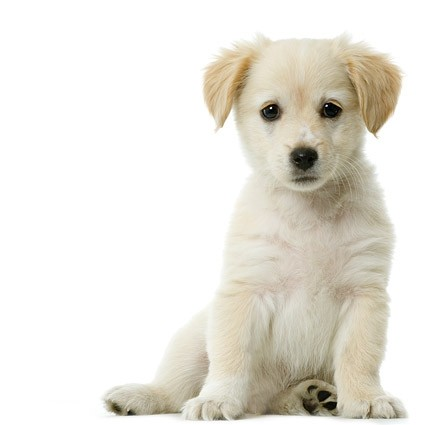
\includegraphics[width=1\textwidth]{img/dog.jpg}
	\caption{output}
\end{subfigure}
\caption[Short title:group delay]{One pulse through the other with group delay}
\label{fig:example}
\end{figure}
Referencing the figure is like always, please see Fig. \ref{fig:example}.


\newpage %For forcing the following text on the next page

\section{Setup and Measurements}
This is now your job....
Do you want to cite your work, because they have influenced you \cite{einstein1905} and \cite{planck2000}.
Test this.


\section{Results}
\label{sec:results}

% a table example .... 
\begin{table}[h]
\caption{ Tables are sometimes needed}
\begin{center}
\begin{tabular}{l|lll}
\hline
City & Distance & weather & Comments \\ 
\hline \hline
Hamburg & 0 km & fresh wind  & too cold\\ 
Bremen & 98 km & also fresh wind  & \\ 
New York & 6548 km & hot & too hot  \\ 
\hline 
\end{tabular}
\end{center}
\label{default}
\end{table}%


% How to itemize: 

A typical day at DESY

\begin{itemize}
\item{8:45 running to the lecture hall }
\item{9:00 start of lecture - speaker is also a bit tired }
\item{12:00 lunch in the cantine - terrible again!! }
\item{13:00 trying to understand what my supervisor is trying to tell me}
\item{17:00 Strandperle - ok, this was not typical due to weather ....} 
\end{itemize}




\section{Summary, Conclusions and Outlook}
Just write it...

% This section should not get a number...
\clearpage
\section*{Acknowledgement}
I would like to express my appreciation of the great help from my supervisors Mrs. Desy and the whole ATLAS group. Technical support from Dr. Faust is acknowledged. Special thanks go to DESY summer student organizers.

% Here starts the section for the references - put references here whenever you quote something, don't
% safe this for later as you will never have time for this 
\begin{thebibliography}{99}

\bibitem{planck2000}
M. Planck (2000), 
{\em Is it real?}

\bibitem{einstein1905} 
A. Einstein (1905), 
{\em \"Uber einen die Erzeugung und Verwandlung des Lichtes betreffenden heuristischen Gesichtspunkt.} Journal  



\end{thebibliography}

\end{document}
